\documentclass[12pt]{article}
\usepackage[a4paper,margin=.5in]{geometry}
\usepackage{graphicx}
\usepackage{booktabs}
\usepackage{listings}
\usepackage{color}

\definecolor{dkgreen}{rgb}{0,0.6,0}
\definecolor{gray}{rgb}{0.5,0.5,0.5}
\definecolor{mauve}{rgb}{0.58,0,0.82}

\lstset{frame=tb,
  language=Python,
  aboveskip=3mm,
  belowskip=3mm,
  showstringspaces=false,
  columns=flexible,
  basicstyle={\small\ttfamily},
  numbers=none,
  numberstyle=\tiny\color{gray},
  keywordstyle=\color{blue},
  commentstyle=\color{dkgreen},
  stringstyle=\color{mauve},
  breaklines=true,
  breakatwhitespace=true,
  tabsize=3
}
%\usepackage{subfig}
\usepackage{subcaption}
\usepackage{hyperref}
\hypersetup{
    colorlinks=true,
    linkcolor=blue,
    filecolor=magenta,      
    urlcolor=cyan,
    pdftitle={Overleaf Example},
    pdfpagemode=FullScreen,
    }
\newcommand*{\figuretitle}[1]{%
    {\centering%   <--------  will only affect the title because of the grouping (by the
    \textbf{#1}%              braces before \centering and behind \medskip). If you remove
    \par\medskip}%            these braces the whole body of a {figure} env will be centered.
}
\title{Homework 3 Writeup}

\author{Tylman Michael\\CSE 546 Machine Learning}
\date{2/18/2023}
%moderncv theme
\usepackage[utf8]{inputenc} 
\begin{document}
\maketitle{}
\section{Cross-Validation Optimal Parameters and Testing}
\subsection{Prelude}
For this homework, I set out to better understand the GridSearchCV functionality of sklearn and how to utilize it for 
deeper analysis. My reasoning was that the burden of proof for professional/research applications of a GridSearchCV must be higher
than the burden of proof for conclusions required for a class. If that's the case, and GridSearchCV was likely made for 
use in a professional/research setting like the rest of sklearn, then it must be possible to do quality analysis using 
this function. So, for every item listed in here, I am only doing operations on either the GridSearchCV, or a single estimator pulled
from the GridSearchCV.

I will also list a single table with the best results (with the param lists cut) for every model for ease of reference 
in Table \ref{table1}. The most important rows to recognize are the last few, where best\_final\_test is the accuracy 
of the best\ model on the test set, best\_cv\_test and best\_cv\_train are the average test accuracies of the best model
 across the CV splits for test and train respectively. A couple of those values are available earlier in the table as well,
 but I included them at the all together for ease of use.
\begin{table}
  \resizebox*{.95\textwidth}{!}{\begin{tabular}{lllllll}
\toprule
{} &                   stack &                  NBbag &                 mlpbag &                  NBada &                treeada &                  SVMbag \\
\midrule
Index                       &                       2 &                    867 &                     14 &                     51 &                     47 &                      17 \\
mean\_fit\_time               &      1405.5506918430328 &     40.285290360450745 &      579.3783206343651 &     102.77094876766205 &      1229.745915234089 &      129.07705068588257 \\
std\_fit\_time                &       56.74206058134601 &     0.6317175670817758 &      7.455601391413241 &     0.8867015999451987 &     1.8724155730382983 &       9.796660667519168 \\
mean\_score\_time             &      11.178422927856445 &      51.00288212299347 &     0.5981229543685913 &     48.676812052726746 &      3.830958664417267 &      27.196506679058075 \\
std\_score\_time              &       1.405742496910865 &     1.8923625091969507 &    0.11387845129075089 &     1.8198226356237728 &    0.28462153313195493 &       4.294021210732005 \\
mean\_test\_accuracy          &                    0.79 &     0.5754999999999999 &                0.79525 &                  0.637 &                0.54825 &                 0.77575 \\
std\_test\_accuracy           &   0.0022360679774997916 &   0.019868316486305507 &   0.008525696452489974 &    0.01383835250309806 &     0.0067961386095341 &     0.00831790237980707 \\
rank\_test\_accuracy          &                       5 &                     44 &                      1 &                      1 &                      1 &                       2 \\
mean\_train\_accuracy         &      0.9977499999999999 &                0.62925 &     0.9940833333333333 &     0.8125833333333333 &                  0.764 &                 0.99425 \\
std\_train\_accuracy          &   0.0007592027982620297 &   0.004872684635347887 &  0.0009537935951883014 &    0.01061281981588514 &    0.01018713785995741 &   0.0008620067027324092 \\
mean\_test\_f1\_weighted       &      0.7912570496724283 &     0.5858494831502836 &     0.7949238630429338 &     0.6431246854754509 &     0.5576218846400178 &      0.7762111731817483 \\
std\_test\_f1\_weighted        &   0.0029872474406088608 &    0.01903181076309097 &   0.008385994462715676 &   0.012909250517893546 &   0.007753848653095678 &    0.009018811244895598 \\
rank\_test\_f1\_weighted       &                       3 &                     38 &                      1 &                      1 &                      1 &                       2 \\
mean\_train\_f1\_weighted      &      0.9977507823245164 &     0.6389193533117794 &     0.9940841593977978 &     0.8137017737836371 &     0.7653651061845691 &      0.9942576816522287 \\
std\_train\_f1\_weighted       &   0.0007583764213535456 &   0.005289021391854054 &  0.0009541156349656866 &   0.010307792046297188 &   0.010124753277141824 &   0.0008584699193975221 \\
mean\_test\_roc\_auc\_ovr       &      0.9730999015536933 &     0.9088672548387857 &     0.9749867328830162 &     0.9364586653065938 &     0.8743949551758458 &      0.9688421608215558 \\
std\_test\_roc\_auc\_ovr        &    0.000915550433627727 &   0.006604637647041263 &  0.0008938521311151068 &  0.0030788513632281837 &  0.0034540071161737835 &   0.0019750940256677376 \\
rank\_test\_roc\_auc\_ovr       &                       1 &                      1 &                      1 &                      1 &                      1 &                       1 \\
mean\_train\_roc\_auc\_ovr      &      0.9999612015765678 &     0.9389531956927522 &     0.9999600333256833 &     0.9844012423207428 &      0.949929571828595 &       0.999923288362849 \\
std\_train\_roc\_auc\_ovr       &  2.4671281578632394e-05 &  0.0030594180625836366 &  1.558742578374733e-05 &  0.0010215200718514444 &   0.002438923495362692 &  3.1182187144615235e-05 \\
best\_final\_test\_accuracy    &                    0.96 &                  0.602 &                  0.961 &                   0.75 &                  0.714 &                   0.791 \\
best\_final\_test\_roc\_ovr     &      0.9989464604987599 &      0.927274695189538 &      0.996860066599987 &     0.9706142287135784 &     0.9326248076880352 &      0.9701864899787338 \\
best\_final\_test\_f1\_weighted &      0.9600616632865854 &     0.6136405868499072 &     0.9609942113384318 &      0.752537870834654 &     0.7160316970317154 &      0.7909626666332018 \\
\bottomrule
\end{tabular}
}
  \caption{Best Results and MetaData}
  \label{table1}
\end{table}

\subsection{Gradient Boosted}
For the Gradient Boosted (GB) classifier, I gridsearched combinations in the learning rate, loss function, and number of estimators.
For the learning rate, I did a linspace of (.01, 2, 25). For the estimators I went from 100 to 700 in steps of 100. And 
for the losses I chose log loss or exponential options. The resulting performances is shown in Figure \ref{figure1}

The shaded regions in the two plots show that learning rate had a much stronger influence on the performance of the model 
than the number of estimators. Interestingly, the training performance of the two loss functions actually inverts when 
we group by estimators or learning rate. In both cases; however, the exponential bests the log loss function in the 
test case.
\begin{figure}
  \begin{subfigure}{.5\textwidth}
  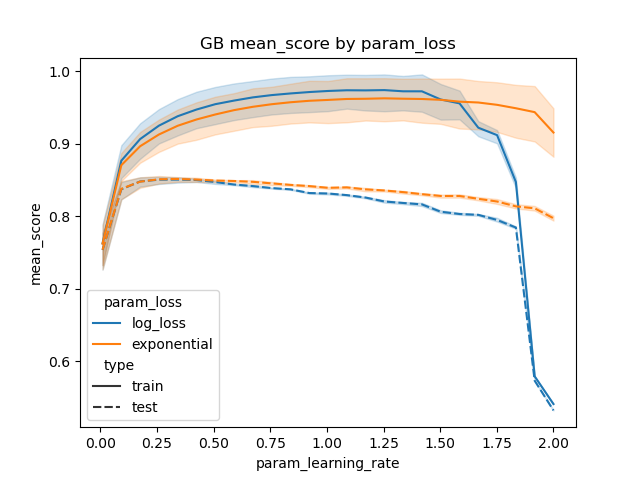
\includegraphics[width=.95\textwidth]{../results/gb/param_loss_mean_score_param_learning_rate.png}
    \caption{Performance VS learning Rate}
    \end{subfigure}%
  \begin{subfigure}{.5\textwidth}
  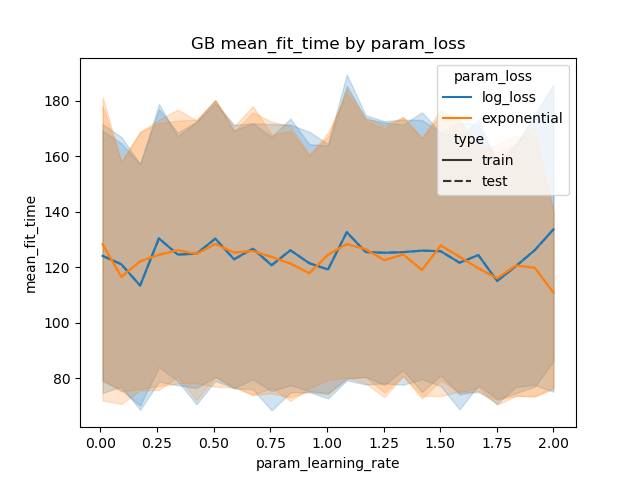
\includegraphics[width=.95\textwidth]{../results/gb/param_loss_mean_fit_time_param_learning_rate.png}
    \caption{Time VS learning Rate}
  \end{subfigure}
  \begin{subfigure}{.5\textwidth}
    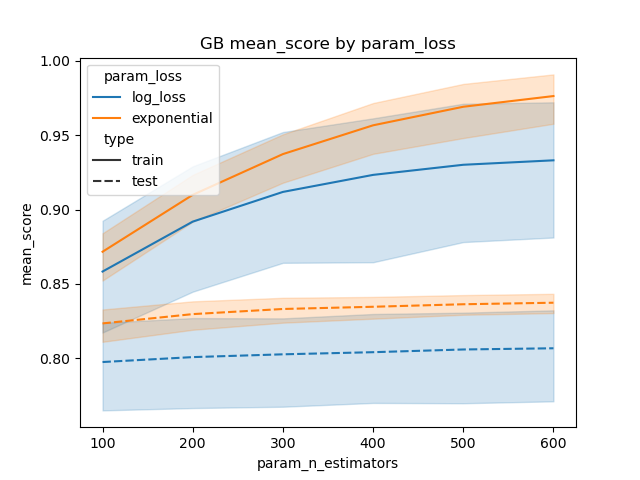
\includegraphics[width=.95\textwidth]{../results/gb/param_loss_mean_score_param_n_estimators.png}
    \caption{Performance VS Estimators}
  \end{subfigure}%
  \begin{subfigure}{.5\textwidth}
    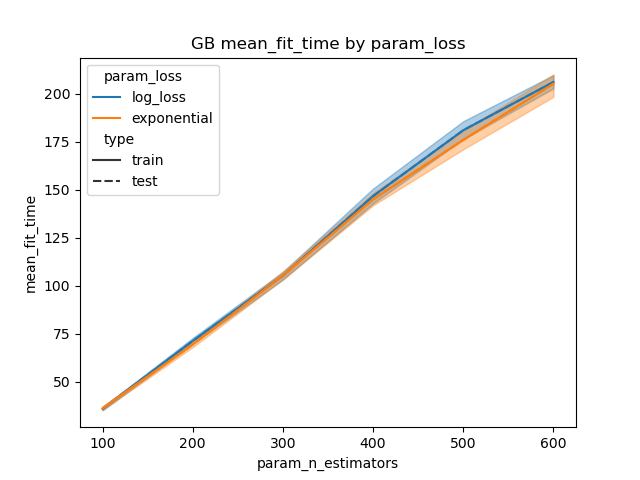
\includegraphics[width=.95\textwidth]{../results/gb/param_loss_mean_fit_time_param_n_estimators.png}
    \caption{Time VS Estimators}
  \end{subfigure}
  \caption{GB Performance and Time}
  \label{figure1}
\end{figure}

The best parameters for all of the parameters were: {'learning\_rate': 0.25875, 'loss': 'exponential', 'n\_estimators': 600} 
which gave the results we can see in Table \ref{table1}. The final test accuracy was very slighly higher than the average
cross validation test performance, but by only a small margin. This model appears to have generalized very well, and shows
only a little bit of overfitting at this stage. Interestingly, the choice in loss function appears to have directly helped
overfitting by lowering the training score and raising the testing score.

Another interesting phenomenenon is that the testing score appears to be much more stable than the training score for both
loss functions, with the exponential loss function being more stable than the log loss function when we group by the number 
of estimators. 

The GB model performed quite well, but I have to acknowledge the training time. I will cover this in more detail in the
conclusion where I decide the best model, but the GB model trained exceptionally slow when compared to the other models.
As expected, the learning rate had no discernable effect on the training time of the GB model, and the training time scaled
linearly with the number of estimators used. However, the slope of this line is the most significant by far of any of the 
other models.

\subsection{KNN}
For the KNN classifier, I gridsearched combinations in the Distance metric and the number of neighbors. 
The number of neighbors varied from 1 to 100, and the Distance metric could be 'uniform','distance' or a 
custom Radial Basis function. I did not also loop over the possible parameters for the rbf, since including it was a
bonus in it's own right. The resulting performance and time complexity is shown in Figure \ref{figure2}.



\begin{figure}
  \begin{subfigure}{.5\textwidth}
    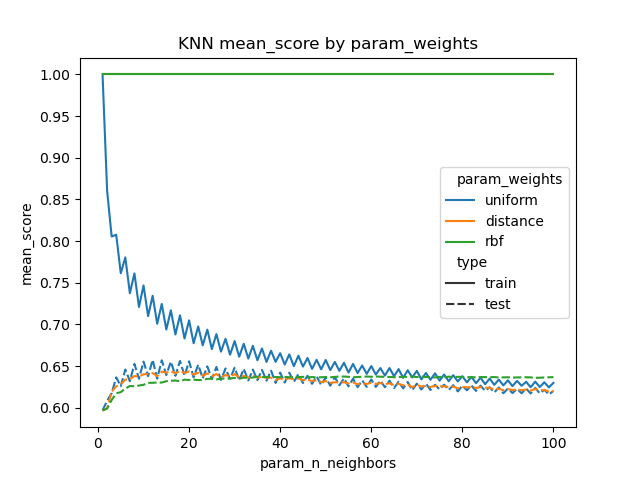
\includegraphics[width=.95\textwidth]{../results/knn/param_weights_mean_score_param_n_neighbors.png}
    \caption{KNN Performance VS N Neighbors}
    \end{subfigure}%
  \begin{subfigure}{.5\textwidth}
    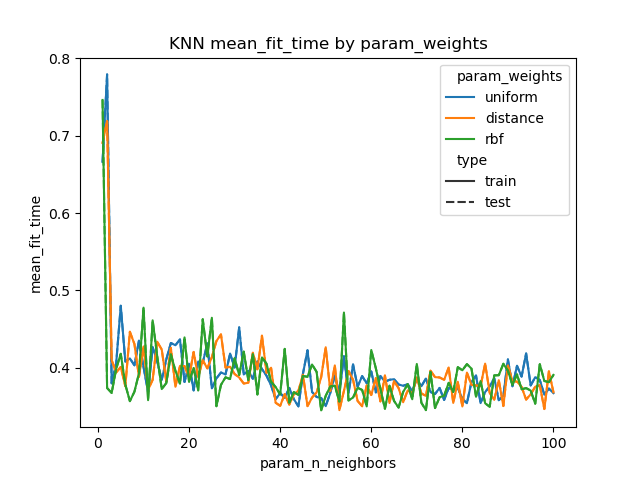
\includegraphics[width=.95\textwidth]{../results/knn/param_weights_mean_fit_time_param_n_neighbors.png}
    \caption{KNN Time VS N Neighbors}
  \end{subfigure}
  \caption{RF Performance}
  \label{figure2}
\end{figure}


This plot shows that the distance and radial basis functions drastically increased training accuracy to be 100\% at all 
values, but did not have a dramatic impact on test performance. This leads me to the conclusion that the non-uniform 
weighting increases the complexity of our models which opens us up to overfitting.

Interestingly, the uniform parameter showed a stairstep behavior where the even number neighbor counts outperformed
the next and previous odd-number amount of neighbors. That's something that caught me by surprise, and I can't quite explain.
This behavior worked in the favor of the uniform distribution, allowing it to peak higher than the other weights. So, 
the best parameter for the weight was the uniform option, which gave better test scores and showed less overfitting.

The best parameter for n\_neighbors was less intersting. We can see that it peaks pretty early in the low 10s, with 
the best parameter being achieved at n\_neighbors = 12, which gave us our final results shown in \ref{table1}.

The best KNN model generalized well, with the accuracy on the test group being quite close to it's average test performance on the 
validation splits during training. It did perform noticeably higher on the training set, but not to a degree which would 
be indicative of oppressive over-fitting. All in all, I'd say the KNN model performed quite well, but trails behind the 
GB model in performance.

The time complexity for the KNN model is uninteresting, but I included the plot here for consistency with the other models. 
Since the KNN model is so simple, we don't have many conclusions to make regarding the time complexity, except when compared 
to other models.


\subsection{Random Forest}
The Random Forest (RF) classifier was gridsearched over the options: max depth, number of estimators, and max features.
The maximum depth went from a range of 10 to 100 with steps of 10, and I also appended a 'None' option which did not 
limit the max depth at all. The number of estimators used a range of 100 to 1000 with a stepsize of 50. Finally, 
the number of features was selected from the sqrt and log2 options.

We can see from Figure \ref{figure3} that the log2 feature selection outperformed the sqrt feature selection at almost
every step. Interestingly, we can see much more consistency when we plot the score vs max depth instead of the estimators,
even though the max depth has more items it is averaging over.  I believe that is evidence to suggest the maximum depth 
has a stronger influence on the performance than the number of estimators.

The best parameters for the RF classifer were: {'max\_depth': 70, 'max\_features': 'log2', 'n\_estimators': 850}, 
which makes sense given the positive trend we are seeing in both of these plots. Unfortunately, if you look at Figure 3: (a)
you'll see that the testing accuracy actually plateaus much faster than the training accuracy, and that this selection
is well into the region where we would consider it to be maximum overfitting of the model since the training accuracy is 1.

However, even though the training accuracy is 1 while the validation accuracy is only .846, we do see that the random Forest
still generalized well to give us a final test accuracy of .844. While we might be tempted to say this is a victory, if we 
look at the greater context of all our models, we can see that this is the only model which showed noticeable loss in 
performance when transitioning to the test set. Two of our models actually increased performance during the switch, and 
the other model only lost .00012 performance, which is entirely neglible. While the loss of performance for the RF 
is quite small, and likely neglible, I think it isn't an accident that the model which shows the most signs of classic 
overfitting is the model which shows the largest drop in performance by a wide margin.

\begin{figure}
  \begin{subfigure}{.5\textwidth}
  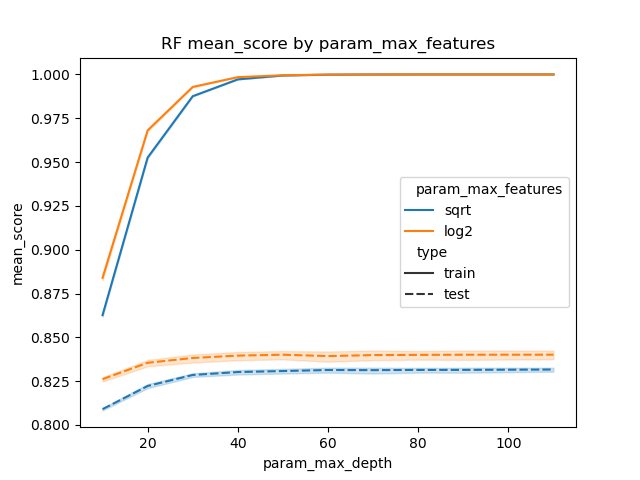
\includegraphics[width=.95\textwidth]{../results/rf/param_max_features_mean_score_param_max_depth.png}
    \caption{Performance VS Max Depth}
    \end{subfigure}%
  \begin{subfigure}{.5\textwidth}
    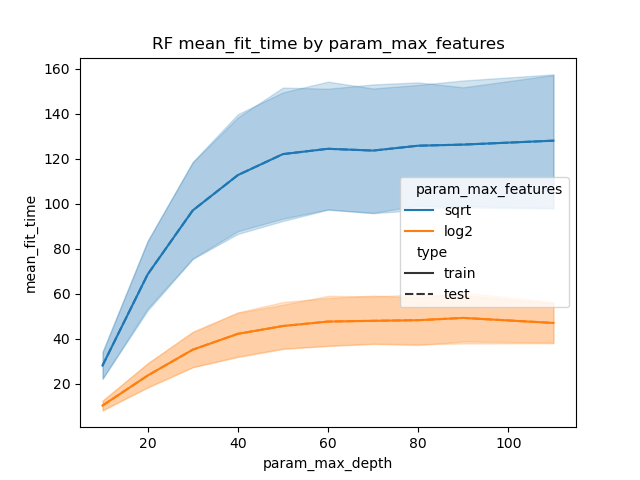
\includegraphics[width=.95\textwidth]{../results/rf/param_max_features_mean_fit_time_param_max_depth.png}
    \caption{Time VS Max Depth}
  \end{subfigure}
  \begin{subfigure}{.5\textwidth}
    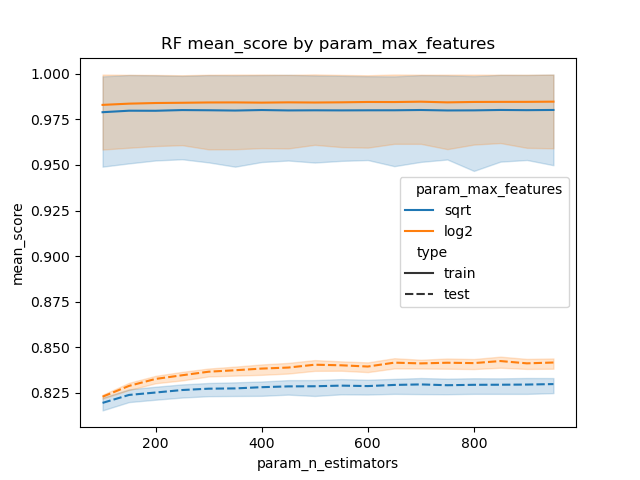
\includegraphics[width=.95\textwidth]{../results/rf/param_max_features_mean_score_param_n_estimators.png}
      \caption{Performance VS Estimators}
      \end{subfigure}%
  \begin{subfigure}{.5\textwidth}
    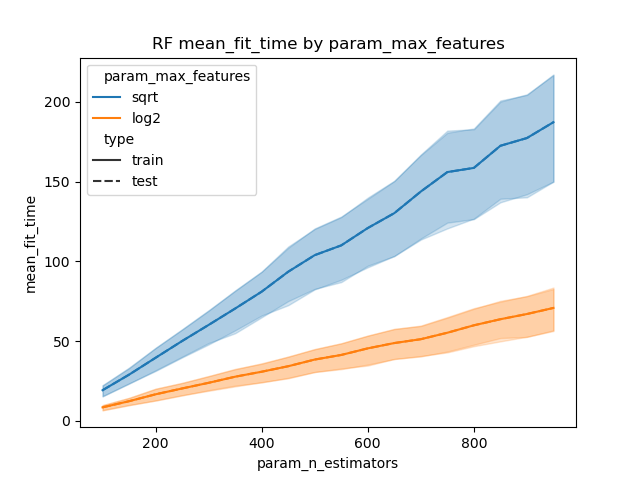
\includegraphics[width=.95\textwidth]{../results/rf/param_max_features_mean_fit_time_param_n_estimators.png}
    \caption{Time VS Estimators}
  \end{subfigure}
  \caption{RF Performance and Time}
  \label{figure3}
\end{figure}

The time complexity of the RF model is very satisfying. The time complexity grew logarithmically with max depth, and 
linearly with the number of estimators. For both of these, the log2 feature selection is better than the sqrt feature 
selection, which is as expected. I want to point out that the absolute worst performing time complexity of the RF with 
a number of estimators of 800 is still better than the GB classifier with 600 estimators.




\subsection{Naive Bayes}
Before we continue, I must declare my bias towards the Naive Bayes (NB) classifier. I find this model to be mathematically
pleasing, easy to understand, elegant, and efficient. If I have two classifiers performing similarly, and one of them is a NB 
classifier, I will almost always pick the NB classifier. 

I used a more simple gridsearch for the NB classifier which altered the fit\_prior option between False and True, and 
ranging alpha from .01 to 5. Interestingly, the fit\_prior option appeared to do nothing for this dataset, and no option
significantly effected the training time. From those two things, the available analysis of the NB classifier is quite 
dry compared to the others.

\begin{figure}
  \begin{subfigure}{.5\textwidth}
  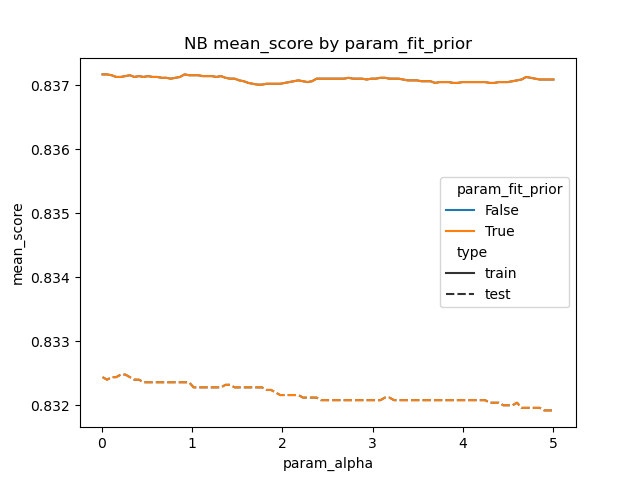
\includegraphics[width=.95\textwidth]{../results/nb/param_fit_prior_mean_score_param_alpha.png}
    \caption{Performance VS Alpha}
    \end{subfigure}%
  \begin{subfigure}{.5\textwidth}
    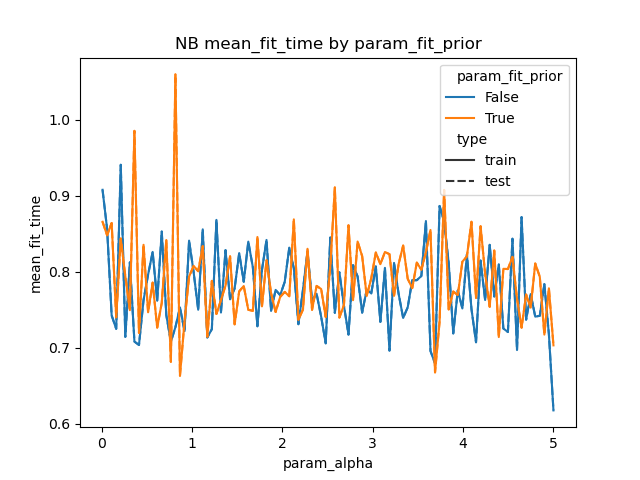
\includegraphics[width=.95\textwidth]{../results/nb/param_fit_prior_mean_fit_time_param_alpha.png}
    \caption{Time VS Alpha}
  \end{subfigure}
  \caption{RF Performance}
  \label{figure4}
\end{figure}

The best parameters for the NB classifier are: {'alpha': 0.2116, 'fit\_prior': True}. The final performance of the NB 
classifier showed absolutely zero overfitting, and nearly perfect generalization. The CV training accuracy was .837,
CV test accuracy was .832, and the final tets accuracy was .832. Furthermore, it did all of this while being trained 
in a time comparable to the KNN classifier. This result is beautiful and evidence of why I have such a strong bias toward 
the NB classifier.

\section{Feature Importance and Missclassifications}

I decided it would be most useful to compare the feature importance between the RF and GB classifiers, and the 
positive/negative importances of the NB classifier. I'll include these results with an interactive .html plot in my 
submission if you'd like a closer look. 

\begin{figure}
  \begin{subfigure}{.5\textwidth}
  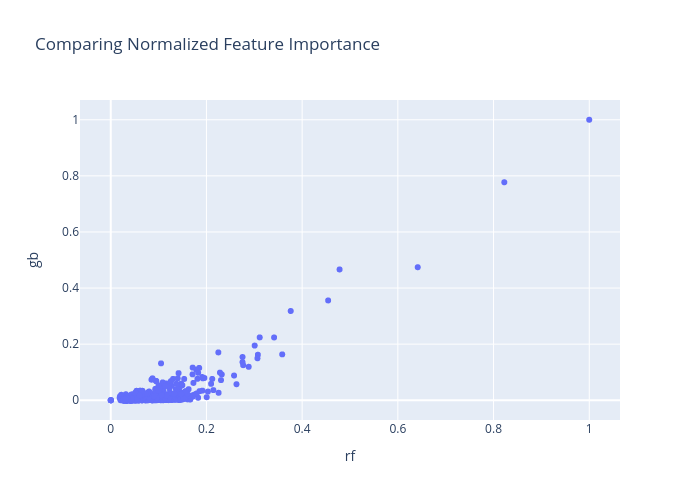
\includegraphics[width=.95\textwidth]{../results/tree_comparison.png}
    \caption{Tree feature importance comparison}
    \end{subfigure}%
  \begin{subfigure}{.5\textwidth}
    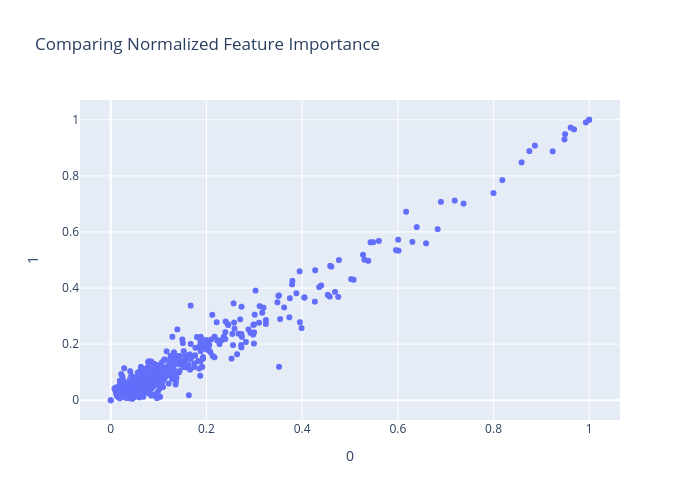
\includegraphics[width=.95\textwidth]{../results/nb_comparison.png}
    \caption{NB feature likelihood comparison}
  \end{subfigure}
  \caption{Feature comparison}
  \label{figure5}
\end{figure}

For the tree-based items, they both agree that Feature 78 is the most important feature by far, with several other features
sharing similar importance. The GB model was much more likely to crush feature importance down to zero than the random 
forest, causing our scatter plot to be skewed below the line y=x. 

For the NB classifier, there is one major outlier of Feature 3. Feature 3 the least important feature of any 
of the models, scoring a 0 importance fot the GB and RF models. All models agree feature 3 is apparently worthless, by a
significant margin compared to the other features. The major reason why Feature 3 confuses me so much is that the 
readme states they took the 1000 most frequently used words, and looking at the likelihood plot of the NB classifier 
enforces the idea that they were sorted at least weakly by their usage. The interactive .html file shows that the 
items with the highest agreement between positive and negative samples are the earlier features. This explains 
why the trees do not show these items to be necessarily important, but it is odd to me that feature 3 appears to be 
entirely unused.

I did not attempt to analyze missed samples from these Three Models. since the data is obtuse to human comprehension. I.E.
I have no idea what feature 78 is supposed to be, or why it was so important. Likewise, I can't tell you meaningfully why 
one sample was missclassified over another without the conclusion being "it didn't fit the learned distribution," which 
we already know. I have no way of providing a meaningful discussion of \emph{why} it didn't fit the distribution without 
knowing what the features should be.

For these same reasons, I decided to look at the missclassified samples as a whole and try to understand the behavior.
So, in Figure \ref{figure6} I took the average distance from all neighbors for each sample, and sorted them from shortest 
distance to longest distance. The resulting plot shows a very interesting behavior. It seems like we don't start seeing a 
significant amount of misses until over double the distance of the very first missed item. Likewise, the largest outliers
see a significant increase in the rate of growth of their average distance. I believe this is a sign of a healthy model 
where the most significant offenders are more likely to be outliers than well-clustered samples.
\begin{figure}
  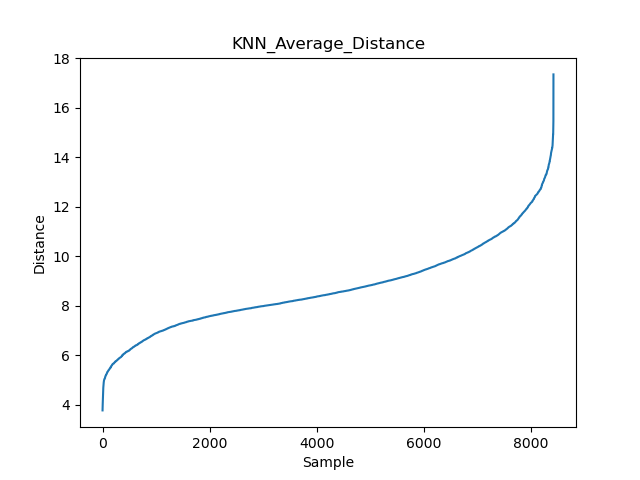
\includegraphics[width=.95\textwidth]{../results/knn/KNN_Average_Distance.png}
  \caption{KNN Missed Average Distances}
  \label{figure6}
\end{figure}

\section{Conclusion and Final Model Selection}

My selection for the best model is the Naive Bayes classifier. I understand that the Random Forest and Gradient Boosted
classifiers have better performance, but both of them come at a cost. The GB classifier trained in about 250x the time that 
the NB classifier took, while showing a much larger amount of overfitting, all for a 3\% increase in accuracy. Likewise,
the RF classifier had even more overfitting than the GB, and it had less performance than the GB classifier. It's saving 
grace is that it only took 100x longer to train than the NB classifier, but still not worth it to take that much longer 
to train to gain a whopping .012\% better performance. 

The explainability of the NB classifier is also comparable to the explainability of both of the other competitive models.
KNN does beat the NB classifier in explainability, but it's the worst in terms of performance by a far enough margin to not 
be in the running for best model in my book. 

Overall, if I had to implement one of these four models for a project, especially if that project needed quick runtime, 
I would choose the NB classifier.


\end{document}